\documentclass[10pt]{sigplanconf}

% The following \documentclass options may be useful:
%
% 10pt          To set in 10-point type instead of 9-point.
% 11pt          To set in 11-point type instead of 9-point.
% authoryear    To obtain author/year citation style instead of numeric.

\usepackage{amsmath}
\usepackage{graphicx}
\usepackage{fancyvrb}
\usepackage{multirow}
\usepackage{url}
\usepackage{hyperref}
\usepackage{breakurl}
\usepackage{caption}
\DeclareCaptionType{copyrightbox}

\begin{document}

\conferenceinfo{SPLASH'11 Companion,} {October 22--27, 2011, Portland, Oregon, USA.}
\CopyrightYear{2011}
\copyrightdata{978-1-4503-0942-4/11/10}

\titlebanner{Wavefront Paper}        % These are ignored unless
\preprintfooter{The Infusion IoC System}   % 'preprint' option specified.

\title{To Inclusive Design Through Contextually Extended IoC}
\subtitle{Infusion IoC, a JavaScript library and mentality for delivering accessible and maintainable systems}

\authorinfo{Antranig Basman}
           {Fluid Project, OCAD University, Toronto, Canada}
           {antranig.basman@colorado.edu}
\authorinfo{Clayton Lewis \and Colin Clark}
           {University of Colorado, Boulder/Fluid Project}
           {clayton.lewis@colorado.edu/cclark@ocad.ca}

\maketitle

\begin{abstract}
Using current software development techniques, code and designs are often unmaintainable from the point of inception. Code is brittle and hard to refactor, hard to press to new purposes, and hard to understand. Here we present a system aimed at creating a model for {\it scalable development}, addressing this and several other critical problems in software construction. Such an aim is far from new, and has resembled the aims of each generation of software methodologists over the last 50 years. It deserves comment why these aims have so signally failed to be achieved, and we will present arguments as to why the combination of techniques explained here could expect to lead to novel results. 

Software products of today are notoriously unadaptable. An application which meets need $A$ generally cannot be extended to meet apparently very similar need $A'$ without something resembling ``software engineering''. Applications present users with a ``take it or leave it'' proposition --- if the software doesn't happen to meet a user's needs or preferences, there's no way to change it without writing more code, which is out of reach for most users. Indeed, software regularly fails to be easily adaptable to meet the needs of users with differing needs, such as in the case of accessibility. These ``precarious values'' --- accessibility and usability with different devices, languages, and personal needs --- are typically left until the end or ignored, and represent a significant expense in traditional approaches to software development. Often these needs are met by developing a largely unrelated version of the application, requiring maintenance of additional, separate code bases. 

Our aim is to enable {\it Inclusive Design}\cite{inclusive-design}, whose objective is to satisfy the needs and desires of the broadest range of users possible. Every designer sets out with this objective to a certain extent, but as well as limitations of intent, there are also strong limitations placed by the technology and economics of software development. Due to the poor scaling characteristics of current techniques, even meeting one set of relatively inflexible needs can be an expensive undertaking, especially over the long term.

To address these problems of adaptability, we present a model for software construction, together with a base library, Fluid Infusion, implemented in the JavaScript language. Fluid Infusion implements an {\it Inversion of Control} model, Infusion IoC, which features a notion of {\it context} as the basis for adaptability, resolved in a scope modelled in terms of a data structure, a {\it component tree} expressing the computation to be performed. In the Context-Oriented Programming community\cite{cop2005}, this model of scoping is known as {\it structural scoping}. We will also work with a model of {\it transparent state} in which all modifiable state of interest to users is held in publicly visible locations, indexed by path strings. This model for state is isomorphic to that modeled by JSON\cite{crockford}, a well-known state model derived from, but not limited to, the JavaScript language. Instantiation in the model is handled by an {\it Inversion of Control} system extended from the model of similar system such as the Spring Framework or Pico first developed in the Java language. 

We relate such systems to goal-directed resolution systems such as Prolog, and show that they have beneficial properties such as {\it homoiconicity}\cite{mcilroy} which have not been seen in a strong or widespread form since the days of LISP. We exhibit some cases to show how the framework enables, through a simple declarative syntax, types of adaptation and composition that are hard or impossible using traditional models of polymorphism. We also relate Infusion IoC to other software methodologies such as {\it Aspect-Oriented Programming} and {\it Context-Oriented Programming} which have been found to greatly increase flexibility and expressiveness of designs. We conclude with some remarks on the applicability of the system to the parallelisation of irregular algorithms, and its relationship to upcoming developments in the ECMAScript 6 language specification.

\end{abstract}

\keywords
JavaScript, Inversion of Control, Transparent State, Accessibility, JSON, Context-oriented Programming

\section{The Development and Need for Inversion of Control systems}

The core of the system described here is an ``Inversion of Control'' system implemented in the JavaScript language. It constructs applications from trees of components expressed declaratively in JSON notation. Whilst the primary use of the system is in assembling user interface markup and operating logic for HTML web applications, these ideas can be adapted to other domains, illuminating broad issues of software construction. We begin by examining the history and motivation of similar systems, the relationship of our IoC system to other models of software construction, and then finish by describing some current applications, and planned future work.

\subsection{The Crucial Nature of Dependency Structure in Software}
\label{sec:lakos}
In a pioneering work, John Lakos\cite{lakos} identified the patterns of {\it dependency} of parts of a software system on other parts as key determinants of software quality. In his conception, a piece of code A has ``knowledge of'' or ``dependency on'' another, B, if names in B appear in A. To mark our technical uses of these concepts, we will qualify them by referring to ``L-dependency'' or equivalently ``L-knowledge''.  In the C++ language in which Lakos was working, there are various gradations of this knowledge, for example, whether the knowledge about B was sufficient to affect the memory layout of objects allocated in A, or merely required the compiler to have visibility of B names when compiling A code. Although the details differ, the core of this formulation is invariant across essentially all programming languages. 

Lakos argued that code in a ``dependency-correct'' system should form a {\it directed acyclic graph} (DAG), when expressed in terms of the logical units into which it was divided and the L-dependencies among them. In the C++ language, these logical units were often classes, although he noted that this kind of boundary could be drawn at any level in a system.

Lakos observed that there were many significant consequences of constructing bodies of code with inappropriately arranged L-dependency, following on from his initial effort to control escalating build times in complex systems. Highly interdependent code was harder to understand, harder to test and maintain, and most importantly to our domain of end-users, tended to be extremely brittle over time. Such code imposes unexpectedly huge development costs in responding to seemingly innocuous feature requests.

\subsubsection{Evaluating Physical Design Quality Through Dependence Graphs}
L-dependency problems are easiest to see in cyclic cases, for example, when some part A of a system depends on part B, but part B also depends on A. Consider the problem of testing this system. One would like to find an order of testing for the parts of the system, such that all the parts that A (say) depends on have been tested before testing A. But when there is a cycle in the L-dependency structure, there just is no such order: in the example, B has to be tested before A, but A has to be tested before B.

\begin{figure*}[htb!]
\centering%
\includegraphics[width=13.6cm]{lakos.eps}
\caption{Comparison of Dependence Structures with Different Geometries for 7 components (following Lakos\cite{lakos}, pp.194-195)}
\label{fig:lakos}
\end{figure*}

Even when there are no L-dependency cycles, systems still differ in important ways, reflected in their L-dependency structure. Figure \ref{fig:lakos} contrasts a few different cases of dependency geometry. Each component is labelled with its {\bf level number}, which is the count of all components (including itself) which have L-dependence on that component. At the left is a cyclic structure of the sort we just described. In the centre is shown a system whose dependence graph forms a balanced binary tree, representing a typical reasonably-well factored system. At the right is a system with a horizontal graph, composed of components which have no mutual L-dependency. 

Lakos proposed a measurement of ``quality'' of such a dependence graph, which is the sum of all level numbers in the graph, known as the {\bf cumulative component dependency} (CCD). This measure can be used to compare the quality of the dependence structure of graphs involving the same number of components. Lakos observes that arrangements showing lower CCD numbers are associated with beneficial properties of many kinds. These arrangements correspond to applications which are easier to test, easier to refactor, faster to build, and which offer better opportunities for reuse. We will further observe that CCD numbers that do not ultimately scale linearly in the number of code units form an ultimate barrier to scalable design and ensure that the design will come to be dominated by {\it accidental complexity} (section \ref{sec:complexity}). 

\subsubsection{Consequences of Improving Dependence Structure in Static Languages}

As it turns out, the problem raised by Lakos' recommendations on the organisation of dependencies cannot be fully resolved in C++, or other static languages, at all. We will consider a typical case, of a design where the majority of dependence arcs are caused by L-knowledge resulting from an {\it aggregation} relationship --- in classical object-oriented terms, where, for example, object A {\bf has-a} object B. Consider a hypothetical DAG of dependency-correct code, organised into units of these classes. Take two of these elements, A and B --- in terms of C++, aggregation-derived L-knowledge of class A about class B, would translate into a requirement for objects of class A to bear responsibility for construction of objects of class B, and not vice versa. This knowledge may be pushed into a common ancestor, C --- but wherever it resides, this constructional knowledge cumulates towards the root of the tree, creating a {\it brittle base} to the overall design. 

\subsubsection{Elaboration of the ``brittle base'' problem}

The ``brittle base'' issue we described is best seen as a {\it dynamic} issue, affecting the quality of a design over its entire trajectory from design through to maintenance. At any particular point in time, the naive method of propagating dependencies from place to place across a design with $n$ logical units would require the instantiation in the design of $O(n)$ types with $O(n^2)$ overall information content in order to express the (cumulative) signature contracts between each pair of nodes joined by arcs in the tree. These types express the signatures of callbacks, travelling in the ``upward'' direction from a point in the tree where a dependency is generated, and the signatures of constructors, travelling in the ``downward'' direction down to where a dependency is used.

Faced with this unacceptable proliferation of types, a skilled designer will apply judgement to the overall design and attempt to consolidate dependencies and their points of generation into {\it equivalence classes} of units which may be treated as equivalent (``is-a'') with respect to their dependency transfer characteristics. Whilst they may be to some extent ``Procrustean'' (having unused arguments in some cases, or failing to transfer required ones) these solutions may be of good quality at a particular point in the design trajectory.

A problem occurs when during the ``maintenance'' phase of the design, (or more accurately, simply its ``period of use''), an unexpected user requirement perturbs the situation by requiring an extra dependency transfer. The equivalence mapping previously computed by the designer then is no longer ideal. The design progressively strains under this failure, perhaps even leading to the rejection of such requirements as uneconomic. When the costs are finally paid, the new ideal division of signatures into equivalence classes may not be closely related to the old, leading to large change costs proportional to the entire size of the design. This is an important source of non-linear scaling of engineering costs with respect to requirements. 

\subsubsection{Attempted solutions lead back to the core issue}
Common attempted solutions to this kind of issue in non-dynamic languages involve constructional {\it design patterns}, usually factories. These impose two kinds of penalties. Firstly, the family of products from the factory need to have a common signature, a serious restriction. Secondly, whilst {\it some} type information may be erased at this polymorphic boundary, remanent type information still naturally cumulates upwards in the DAG of knowledge in a way that prevents scaling. In the next section we will explain how a certain kind of framework, known as an {\it Inversion of Control} system, can resolve these kinds of issues, given a sufficiently dynamic base language.

\subsection{Inversion of Control Systems}

The Java language is not particularly dynamic, but enjoys enough of this quality through its reflection system and the possibility for bytecode manipulation that some workable solutions to the fragile base problem emerged, generically described as ``Inversion of Control'' (IoC). Martin Fowler outlines some of the variants of IoC framework in \cite{fowler}; popular frameworks in Java include Pico, Avalon, and currently most popularly the Spring framework\cite{spring}.

The defining activity of such an IoC system, specifically named by Fowler as {\bf dependency injection} is as follows: If an object of class A needs an object of another class B at construction time, rather than A's code calling a constructor for B, A's need for a B is registered in some kind of declarative format with the IoC system. The IoC system then {\bf injects} an instance of B into the object that needs it. The ``inversion'' is that ``asking for an object'' is replaced by ``being given an object''. The operation of such a system relies intrinsically on dynamic properties of the target language. In fact, rather than ``constructing itself'' as is the case in static languages, the entire tree containing A, B and all neighbouring dependencies is constructed by the framework, informing the target code of lifecycle points in a model similar to that of event-driven frameworks. The IoC framework, in this model, takes the place of the brittle constructional code otherwise placed in class A or some higher point of dependency.

Users of these frameworks get increased agility in the face of end-user requests and variability in environment. That is, important environmental decisions (in the concrete terms of workaday developers, issues such as transaction management, database dialect, message resolution etc.) are taken out of the code and replaced by declarative configuration.

As well as resolving the ``brittle base'' problem, IoC frameworks improve the L-dependence structure of a design in a number of ways. Firstly, a choice may be made not to support designs with cyclic dependencies (use of Infusion IoC mandates and assists this, whilst it is a configuration option available with Spring IoC). Secondly, the facilities of the IoC system may flatten the dependence graph of a design by removing a number of arcs, which represent dependencies that would otherwise be manifest in the application design but instead are subsumed into basic framework facilities. More powerful IoC frameworks can remove progressively more dependence arcs from the application design, depending on their idiom and capabilities. 

\subsubsection{Conclusions for scaling of design costs}
\label{sec:iocscale}
We have identified two important routes through which traditional design methods fail to allow the costs of a design to scale linearly with the number of ``function points'' addressed by the design. Firstly, the brittle base problem which is resolved by essentially all IoC systems. Secondly, the tendency of Lakos CCD numbers calculated from the physical design structure to scale faster than linearly. This second point can only be addressed by methodologies which allow the physical design structure to be improved whilst still expressing the same design. For this second point we will return in section \ref{sec:subcomponents} to show how the Infusion IoC system can remove a large number of dependence arrows from a physical design map which corresponded to cases of aggregation and inheritance in a traditional object-oriented (OO) design. Before then, we will consider in section \ref{sec:brooks} the implications of these kinds of superlinear scaling for the scale of economic benefits that could be realised through different choices of methodologies.

\subsection{Limitations and Extensions to the IoC model}

A significant lack in existing IoC systems is a suitably flexible concept of {\it context}. To a Java IoC system, the context is a static piece of configuration (or associated runtime structure) known as a {\bf container}. A configuration file is entered into the system as a global specification and if users or developers require changes in resolution based on recognition of a new context or requirement, they need to change the file. Even organising such files hierarchically does not permit decisions to be made based on dynamic considerations. But we can extend the notion of IoC to allow contexts as well as tasks to shape what a system will do.

The Fluid IoC system supervises the matching of names of functions to implementations. What we speak of as a {\bf function name} is more generalised than the traditional notion of a ``function'' in that it does not necessarily correspond to a function as implemented directly in the programming language. All names of such functions could, however, if registered globally serve as ``function names'' if required. Instead a ``function name'' corresponds to the notion of a ``task to be performed'' in the world of a user. There are generally different classes of ``users'', operating at different levels in a the tower of abstractions, where the definition of a task at the level of one user, say an end user, decomposes it into subtasks that make sense only to a user at another level, say an application designer.

An implementation provider --- and even unrelated third parties --- can provide a set of directives to the IoC system, which specify under which conditions a given implementation is an appropriate one to deliver to an end user. These directives are named {\bf demands blocks}, matching conditions which are represented by supplying one or more {\bf context names}. These names are also simple strings, like function names. 

The power of the system to proceed in a contextually aware way is significantly enhanced by allowing the names of {\it products} of the system to serve as names of {\it contexts} guiding the construction of future products. Some names may serve as both function names and context names. The name of a user interface widget, for example, may be used sometimes to specify needed functionality, and sometimes to specify a context in which a subsidiary widget might be embedded.
\section{Relation to other Programming Paradigms}
\subsection{Link to Goal-Directed Programming}
\label{sec:prolog}
One way of understanding the cascade of instantiations performed by an IoC system in pursuit of constructing a particular component, is as related to the {\it resolution} process performed by knowledge-oriented systems such as Prolog. Prolog casts knowledge in the from of {\bf relations}, connecting one term with another. The input from the user proceeds ``forwards'' in their world, expressing the dependence of one proposition (or alternatively seen, ``goal'') on another. Each rule of this kind is entered into a database of such rules progressively, building up an unbounded network linking these propositions. A run of the system takes the form of requesting the status of a particular proposition --- execution then cascades ``backwards'' (in the view of the developer) through the set of dependent rules until an answer can be determined.

Recursive resolution of dependent components by an IoC system can be seen as a model of a similar process as the cascade of Prolog relation resolution. Important differences are that whilst this IoC system currently operates no form of ``backtracking''; on the other hand, we add a concept of {\bf context} to the resolution system. Absence of contextual awareness was historically a weakness of Prolog, which, for example, provided no straightforward means for dealing with situations which changed over time. 

\subsection{Link to Aspect-Oriented Programming}
\label{sec:AOP}
A popular approach for dealing what it terms ``cross-cutting aspects of a design'' which has grown up alongside and in some cases intertwined with the use of IoC is known as ``Aspect-Oriented Programming'' (AOP). In this model, the implementation domain of a codebase is stratified, forming a higher ``meta-level'' of design comprising units of code (in a related, but usually distinct syntax) which consists of directives which {\it advise} the operation of the remaining base level of code which can then usually enjoy some kind of simplified implementation.

AOP systems are often extremely powerful, and have the ability to issue {\it advice} which modifies the execution of the base code at the level of individual method calls or property access --- either modifying these operations or replacing them entirely. The points where an AOP advice matches or ``joins'' a design are indivually named {\it join points}, described by a specification or query known as a {\it pointcut}. Pointcut expressions take quite low-level forms, usually expressed in a dialect reminiscent of regular expressions. With the data-hiding mentality which goes together with object-orientation (OO), AOP pointcuts usually have quite limited insight into the contextual situation which has been matched. As a result of the very local oversight of the pointcut matching and advice process, AOP designs can become very hard to understand without custom tools.

The execution modification effected at an AOP join point may be considered as a kind of {\bf dispatch}. A more familiar kind of function dispatch is the resolution from the name of a polymorphic function in an OO hierarchy onto a particular implementation held in a derived class. Infusion IoC also implements a form of dispatch by following rules held in declarative structures known as {\bf demands blocks} (see section\ref{sec:demands}). Common across all situations is the progress from a specification of an operation to be performed in the form of a {\it name} to a particular concrete implementation to be used in a particular context.

Infusion IoC has a similar kind of power of dispatch to traditional AOP, since the set of dispatch rules is always {\it open} and {\it external} to the body of code being advised. However, compared to AOP, it is at the same time limited in its scope for matching, as it is broadened in its ability to interpret context. A Infusion demands block can only act at points in a design where the IoC system is already instantiating a subcomponent in the tree, or else where the user has explicitly requested its operation (e.g.\ by means of a suitably declared event or method). However, when it does act, the dispatch modification may make use of the same contextual resolution system which guided its own matching, to stably discover relevant pieces of state over the entire component tree in scope, rather than just those located close to the join point site as in traditional AOP. This tradeoff of increased formality of matching against increased contextual understanding should produce designs which are much easier to understand as a whole, although we still anticipate a very important role for assistive tools. 

\subsection{Relation to Context-Oriented Programming}

A relatively recent innovation, aimed at precisely the weakness of traditional goal-directed languages that we identified in section \ref{sec:prolog}, is that of {\bf Context-Oriented Programming} (COP) \cite{cop2005}. COP can also be seen as a related development to AOP of the previous section, as well as an outgrowth of OOP. In the original formulation of the authors, code held within standard methods in an OO hierarchy is enhanced by definitions of {\bf partial methods} which are aggregated in groups known as {\bf layers}. At the time of execution of the enhanced method, one or more of these layers may be active, leading to a modification of the base method by partial methods held in the active layers. A partial method differs from a standard method in that it contains a control flow point at which it may defer to the original method --- this control flow point is named by the COP authors as {\tt proceed}. The layering of a partial method onto a standard method (or stack of other partial methods) can thus be seen in AOP terms as an {\it around advice} --- when a layer containing such a partial method is activated, it {\it advises} the base method, wrapping it in the control flow held in the partial method. \cite{cop2010} contains more detailed comparison and contrast of COP with AOP. 

Since awareness of context is one of the crucial ways in which our system differs from many previous systems, it is relevant to examine common ground between our system and COP, and also ways in which it differs.

\subsubsection{COP Layering with OOP --- Portability Profile}
COP is explicitly founded upon OOP, since the mechanism of a layer, once activated, is to effect {\it behavioural modification} by advising the workflow of methods in their position in an OO hierarchy. For this reason, COP can be effectively ported to a wide variety of standard OO languages, such as Smalltalk, Java, Python, etc.\ --- \cite{cop2009} contains a survey of such ports extant at 2009. On the other hand, the Infusion IoC system presented here is not based on OO, and relies strongly on base language features which allow manipulation of state held as recursive literals of the language. As a result our system could only easily be ported to languages without a fundamental OO representation and with support for such literals such as LISP and JavaScript.

\subsubsection{COP scoping rules}

COP presents a number of routes for determining when layers should be activated --- \cite{cop2009} mentions a few, such as {\it thread-local} and {\it global} which are supported by our system, and some which are not, such as {\it dynamic extent}-based (block plus call stack-scoped) activation. However, the essential and most fundamental mode of activation of contexts in our system is one which the COP authors, as well as ourselves, name {\it structural scoping}. Structural scoping is described in the COP literature at \cite{cop2010}. Since COP is not cast in terms of structures but instead in terms of objects, structural scoping is presented as an extension to the COP activation model for use in a particular domain (a graphical graph editing application, {\it Morphic}) with activation in practice honoured through dynamic extents in an adaptation library. 

Since our system organises code units (``components'') into a directly--addressed transparent state structure (section \ref{sec:state}), the primary and natural means of context scoping is structural, with the global and dynamic methods held as secondary. The scoping rules are treated in detail in section \ref{sec:scope}. 

\subsubsection{Implicit formation of layers}

Whilst a layer in COP is built up as a self-contained, named unit, the units of context which are activated in our system are built up implicitly through open aggregation. The ``layer'' which is active for a particular dispatch in Infusion IoC is composed just out of those {\it demands blocks} (see section \ref{sec:demands}) which match the names which can be found in the portion of the structure holding the dispatch site which is in scope. Thus our system remains always open for modification by third parties, without requiring access either to a particular layer definition which is in effect, or access to the call stack below the point at which dispatch is to be modified.

\section{Context of the Solution}
\subsection{Domain of Validity}
\label{sec:deep}
It is useful to try to draw out the domain of software tasks for which this approach may be relevant, against a background of tasks for which it may be less helpful. There is a traditional dichotomy drawn between problems which could be named as ``deep'' --- those limited by problem complexity, such as design of a compiler, operating system or database, and others which could be termed ``broad'' --- those limited by problem change and definition, such as the interfaces and implementations of user-facing systems on the web and elsewhere. The system described here is most applicable to the latter type of problem. 

However, this dichotomy itself deserves some comment. Software engineers, and computer scientists, as they are for the most part working surrounded by their peers, tend to arrive at a disproportionate focus on the former, ``deep'' category of problem, the form of problem which they create for themselves and each other. This leads to an exaggerated focus both on the particular kinds of difficulties which these problems pose, and also on their real value in the world. The overwhelming majority of consumers for software artifacts are not programmers --- consisting in the most part of normal human beings wanting some work done --- this work in the most part of some orderly and idiomatic access to some form of shared state in the world. It is actually the norm, rather than the anomaly which software professionals can sometimes take it, for problem definitions to be vague, constantly shifting, and even to themselves comprise a huge domain of variation with respect to the ``market'' --- the full variation of human requirements within the scope of Inclusive Design. We contend that this self-focus by the community has led to the prevalence of and disproportionate value attached to approaches such as the ``data hiding'' strand of the object-oriented philosophy which are actively counterproductive when applied to the vast majority of programming tasks as laid out in our presentation of this dichotomy. Below (in section \ref{sec:state}) we will explain how the antithesis of this approach, which we name {\it transparent state}, is crucial to our formulation of IoC and also to addressing these kinds of tasks in general.

\subsection{Existing Configurable Systems}
\label{sec:configurable}
It is worth examining the most configurable kinds of systems which the industry has so far produced, and explain the kinds of variation which we aspire to express, and why they are essential to any conception of Inclusive Design, beyond the traditional conception of ``accessibility''.

Some highly configurable products are intricate desktop applications, such as Microsoft's Visual Studio or IBM's Eclipse, aimed at developers, and Microsoft Word, a word processing application ostensibly aimed at normal human beings. These offer configurations including the following kinds:
\begin{itemize}
\item Configuration of keyboard bindings used to invoke functions of the application
\item Reorganisation and customization of ``toolbars'' holding icons invoking application functions
\item Alteration of layout and positioning of panes holding working documents, indexes of these documents, menus and toolbars
\item Installation and configuration of ``plugins'' offering extensions to the application's function (for example, the ability to work with different kinds of document, or integrate with a particular kind of remote service)
\item Others
\end{itemize}

Whilst this is a form of ``high water-mark'' in terms of configurable systems, it falls short of what is required for Inclusive Design. There it is essential that very many aspects of an application be modifiable to meet diverse user needs. For example, users with low vision will require quite large type fonts, and may require unusual color contrast; users who do not read well may benefit from rarely used content or controls being suppressed or moved to subsidiary screens. In general, Inclusive Design requires that, as much as possible, all aspects of a user interface be subject to configuration.

In addition to these drawbacks to configuration systems, the reach of the system itself falls short. Here are some kinds of configuration which are desirable, and also capable of expression in a system such as Infusion IoC:
\begin{itemize}
\item Replacing application-wide, a control with a particular function by one with the same data binding function but different presentation and mode of operation --- for example, a numeric bounded range presented with spin buttons replaced by a linear slider
\item Changing interaction idioms over domains with a particular geometry --- for example, items displayed in a linear list which are navigable by means of arrow keys might be customized to allow navigation to wrap from the top to the bottom of the list, or else to ``stick'' at the extremes of the list
\item Reformulating the workflow of portions of an application so that multiple controls displayed in a single, complex dialog are replaced by a linear sequence of simpler steps
\end{itemize}

The customization we are seeking also aims at some broader values --- 
\begin{itemize}
\item To make it as easy as possible to transport customisations from one environment or ``application'' to another whilst preserving as much semantic meaning and function as possible\footnote{This goal is a key goal of one of the major partners of the Fluid Project, the {\bf Global Public Inclusive Infrastructure} (GPII)\cite{gpii} which aims to deliver universal accessibility (and hence universal customization) for all applications, mediated by means of globally available personal profiles held in a cloud-based system}
\item To allow as much customisation as possible to proceed by {\it direct manipulation in context} --- that is, by a modal interaction or otherwise --- to allow the customization of a UI element to be achievable by an operation directly performed on the element itself, rather than in a distant and separately developed part of the UI
\item To achieve this level of configurability with no extra effort on the part of developers --- that is, without requiring them to plan up front for the specific axes of configurability which the resulting application offers\footnote{This is a goal specifically defeated by ``object-oriented'' methodologies which typically cast amenability to a particular form of configuration in terms of derivation from a previously formulated {\it interface} or {\it base class}. New such axes cannot be introduced without rewriting existing code.}
\end{itemize}

These broader values are still distant, but we believe they are only achievable through development organised on the principles we have described for our system, relying on some key choices:

\begin{itemize}
\item Expression of customization as well as application structure in a declarative form based on transparent state --- for which a good model is the state-based JSON dialect of JavaScript, highly amenable to transformation and transmission
\item Interpretation of customization as well as application structure in a {\it context-aware} semantic --- where each configuration item is not only {\it context-aware} but also {\it context-forming} --- that is, forming a context guiding the interpretation of further items.
\end{itemize}

The conjunction of {\it customization} with {\it application structure} in these two goals suggests, as we believe, that a further key element in achieving the goals is the specification of what we call application structure {\em in the same terms as} those we cast what we have called customization. This conjunction has been seen already in configuration-based IoC systems such as Spring and Guice, but so far only in thin layers representing the outermost and grossest layers of application function (and hence those of less immediate interest to end users) and not in a suitably context-aware way.

\subsection{Scale of Potential Benefits}
\label{sec:brooks}

A landmark paper assessing the scale of benefits that might be expected from a new programming methodology or technology was Brooks' ``No Silver Bullet'' \cite{brooks86} of 1986. In it he makes the crucial distinction between {\bf essential complexity} (the complexity inherent in the specification of a particular task to be met by software) and {\bf accidental complexity} (the complexity which the methods and technologies used in the solution add to the task). Through various considerations, Brooks concludes that it is unreasonable to expect more than one order of magnitude in efficiency improvements through a change in methodology. We consider through arguments here that his conclusions are pessimistic and we should expect that very much greater improvements are possible.

\subsubsection{Broadening of the field and redundancy}
The number of practicing software engineers may have exploded more than 100-fold since the 1980s when Brooks was writing. The paradox of this huge explosion of the discipline is that rather than driving the satisfaction of differing needs, (the ``one size fits one'' of Inclusive Design), the average software practitioner finds him/herself mostly involved in makework, integration tasks, or duplicating numerous small pieces of work that have already been performed by his/her peers. This is nowhere more true than in the field of web applications, where millions of apparently very similar widgets and interactions are backed by thousands of different hand-crafted workflows written in standard procedural logic. 

The natural economics of the field will gradually improve this situation over time, as standard frameworks and technologies such as jQuery and HTML5 displace their competitors, but this does not obviate the fact that this massive redundancy of effort harbours the possibility for great increases in efficiency --- at least an order of magnitude through this cause alone.

One reason Brooks may fail to consider the power of the redundancy argument is that at the time of writing, the majority of the work done in the field was still of the type categorised as ``deep'' in section \ref{sec:deep}. That is, this was specialised work in the construction of artefacts such as operating systems, IC design, compilers, and numerical algorithms primarily of interest to computer scientists. Because of more tightly defined requirements, and greater variation in delivery environments, less of the redundancy across projects of this kind is likely to result in realisable savings. 

\subsubsection{Order of essential complexity argument}
\label{sec:complexity}
Brooks accepts that the methods of his day (including the then still nascent object orientation) imply a superlinear scaling of problem complexity with respect to problem size. However, without good reason, he ascribes all of this superlinear scaling to the domain of ``essential complexity'' rather than ``accidental complexity'' --- to quote, {\it ``Many of the classic problems of developing software products derive from this essential complexity and its nonlinear increases with size.''}. He makes no references to superlinear scaling deriving from accidental complexity but instead seems to treat accidental causes as operating simply through proportional effects. In our section \ref{sec:iocscale} considering the effects of dependency in software design, we have presented several causes through which superlinear accidental complexity is certain, using current methods in software technology, and we are aware of many more. Until the field as a whole has identified and removed {\it all} perceptible causes of superlinear accidental complexity, Brooks' assertion that the success of software engineering is limited by essentials is not tenable. So far, arguments in the literature that make direct quantitative assertions about the order of accidental complexity which could be expected from following a particular software model or methodology are not common.

\section{How Infusion IoC is Used}

The configuration for our IoC system is issued in two kinds of JSON structures, known as {\bf defaults} and {\bf demands blocks}. This configuration is {\it static}, in that it is issued directly upon loading of the containing JavaScript files, and does not change over the lifetime of the application. A different value for defaults/demands constitutes a different version of the application or framework in question. Defaults and demands blocks are governed by a well-defined grammar, although at various points in the ``syntax'', the content is unconstrained, to allow arbitrary application structure to be expressed. The named units of composition described by the grammar are named ``components'' although these need not correspond to the traditional concept of a ``UI component'' or ``widget''. 

The examples presented here show the syntax supported by the version 1.4 release of Fluid Infusion, of August 2011. Since the Infusion IoC system is still under development, future versions of Infusion will feature different support, although the basic syntax presented here is expected to remain essentially stable. 

\subsection{Defaults and Components}
\label{sec:defaults}
A {\bf defaults block} sets up a default set of options for a component, as well as defining its immediate composition structure in terms of subcomponents and other non-component material. A run of the IoC system may be triggered by a call to a concrete JavaScript function which directly or indirectly instantiates one or more components in accordance with this configuration, creating a {\it component tree}. Components are {\it instances}, analogous to object instances in an OO system but differing in a number of ways. Points of similarity are that components are packages of related data and functions ({\it methods}) --- differences are that components are considered freely addressible as JSON structures, and are not derived from either classes (in the OO sense) or a prototype hierarchy (in the JavaScript sense). 

Some roles for components in our system are as follows:
\begin{itemize}
\item A generalised ``unit of computational work''
\item An actual ``widget on the screen''
\item The result of a decision about an implementation strategy
\item A context for further such decisions
\item A named unit of scoping where state may be looked up
\end{itemize}

\begin{figure}
\fontsize{7pt}{8pt}\selectfont
\begin{Verbatim}
fluid.defaults("fluid.uploader.multiFileUploader", {
    gradeNames: "fluid.viewComponent",
    queueSettings: {
        fileSizeLimit: 20480,
    },
    ...
    components: {
        strategy: {
            type: "fluid.uploader.progressiveStrategy"
        },
            
        fileQueueView: {
            type: "fluid.uploader.fileQueueView",
            options: {
                model: "{multiFileUploader}.queue.files",
                uploaderContainer: "{multiFileUploader}.container"
            }
        },
   ...
   }
}
\end{Verbatim}
\caption{Sample of a defaults block}
\label{fig:defaultsBlock}
\end{figure}

Figure \ref{fig:defaultsBlock} shows part of the defaults structure for a component {\tt fluid.uploader.multiFileUploader} implementing the UI of a progressively enhanceable Uploader widget. Parts of the configuration similar in nature to that shown are omitted with ellipses. Note that the names of components are qualified names held in a (single) global namespace. Whilst this top-level component is a {\it view component} in the MVC sense, subcomponents further down the tree will in general have more abstract functions and not be bound to the view.

\subsubsection{Grades}
\label{sec:grades}
Firstly, the component announces its {\bf grade} --- grades are forms of {\it types} but a specific conception based around {\it composition of JSON documents} rather than having a focus on runtime data structure or substitutability as in OO. This composition is operated by {\bf merging} the contents of multiple documents which are given the semantics of {\it aligned state}. This is a natural operation on the JSON model of state, as canonically implemented by standard utilities such as {\tt jquery.extend()}. This is closely related to our conception of {\it transparent state} discussed in section \ref{sec:state}, and consequences of this alignment are discussed further in \ref{sec:align}.

The primary purposes of Infusion Grades are to i) fix the signature of the component's creator function, and ii) to set up any special semantics to be applied when building up component specification through merging of JSON structures. This latter amounts to a light {\it schema} applied to the JSON structure of the component's options which is otherwise free-form (e.g.\ in this case, the {\tt queueSettings} section). There are currently only 5 grades built in as primitives the Infusion system itself, named {\tt littleComponent}, {\tt modelComponent}, {\tt eventedComponent}, {\tt viewComponent} and {\tt rendererComponent}, although in fact any component may act as a grade through its {\tt defaults} structure. 

In this way, we create a model for {\bf types as documents} which is crucial to the reduction of all application structure to a declarative form. New types can be created by simply supplying new documents to the system, and the effect of {\it combining types}, often so problematic in the OO world as an unclear pattern of {\it multiple inheritance} can simply be understood in terms of {\it combining documents}. The way is paved for end users to engineer the effect of creating their own ``types'' using straightforward authoring tools, bypassing the traditional ``gatekeepers of state'', the developers.

\subsubsection{Subcomponents}
\label{sec:subcomponents}
The view in Figure \ref{fig:defaultsBlock} shows 2 subcomponents configured for the top-level component, which are named {\tt strategy} and {\tt fileQueueView}. When the component is instantiated, the subcomponents will be constructed by the system and assigned as top-level members of the overall component with these names. An important aspect of this aggregation system is that, since the subcomponents are resolved and instantiated by the framework, there is no necessary induction of L-dependency (see section \ref{sec:lakos}) of a supercomponent on a subcomponent by this form of ``has-a'' relationship as there is in classical OO systems. In classical OO, this dependency is induced by constructional responsibility for the subcomponent by the supercomponent, which here is absent. Indeed, third parties may freely contribute additional subcomponents, or modify or resolve away the subcomponents drawn up in defaults blocks, without necessarily disturbing the operation of the supercomponent, as we will show in section \ref{sec:demands} on {\it demands blocks}.

The subcomponents here are described by {\bf type names} --- these are {\bf function names} in the same space as the supercomponent name {\tt "fluid.uploader.multiFileUploader"}. Note that these {\bf need not} correspond to the names of actual functions globally registered into the system. In this case, {\tt "fluid.uploader.fileQueueView"} does indeed correspond to such a concrete function, whereas {\tt "fluid.\\uploader.progressiveStrategy"} does not. The latter name is supplied as a function name which will enter {\bf function resolution} as described in section \ref{sec:demands}. This contrast may be compared to the contrast between {\it interface names} and {\it concrete class names} in a classical OO system, in that the latter are expected to be directly instantiated, and the former are not --- the situation is not directly analogous since in Infusion IoC there is no necessarily induced ``is-a'' relationship between a function name entering resolution and the concretely resolved name used for instantiation. This is a consequence of the fact mentioned in the previous paragraph, that a subcomponent need not, and in most cases does not, impose any direct contract on its supercomponent.

The typical absence of this upward contract in component hierarchies driven by Infusion IoC is one of the crucial ways in which our system improves the L-dependence structure of a design. By removing these ``dependence arcs'' from the graph, its geometry is pushed further towards the right-hand end of the diagram in Figure \ref{fig:lakos}, representing designs with a flatter, more scalable dependence structure. 

\subsubsection{Context Expressions and Scoping}
\label{sec:scope}

The subcomponent {\tt fileQueueView} which is more concretely defined in Figure \ref{fig:defaultsBlock} includes some configuration using a special syntax, e.g.\ the string {\tt "\{multiFileUploader\}.\\container"}. This type of expression is used extensively within IoC, referred to as {\bf contextualised EL expression} or {\bf path expression}\footnote{The use of {\it expression} here is slightly misleading since in fact no expression elements (operators, variables, etc.) are permitted in these strings. The usage of ``expression'' has been inherited from other environments, such as JSPs, ASPs, etc. where a full {\it expression language} was provided for such string-encoded value references.}. The initial section within braces refers to the name of a {\bf context}, actually resolving onto a particular component in the tree that will instantiate, and the remainder of the expression is interpreted as a path within that component. 

A component can be matched via the {\it context} portion of such an expression through a few routes. In the current system, a component, once instantiated in a component tree, gives rise to either two or three {\it context names} which can match against such a name within braces, e.g. {\tt multiFileUploader} in this case. Considering as an example, the context names formed by the subcomponent {\tt fileQueueView} above are as follows:

\begin{itemize}
\item The fully qualified name of the concrete component as instantiated (in the above case, {\tt fluid.uploader.fileQueueView})
\item The final segment of the fully qualified name (e.g. {\tt fileQueueView})
\item The subcomponent's name within its parent, if any (in this case, {\it also} {\tt fileQueueView}).
\end{itemize}

Such context names are considered {\it in scope} from a site of resolution, for example, the instantiating {\tt fileQueueView} component above, if they match a component which is either an ancestor (container) of the component holding the resolution site, or if they are a sibling of such a component. Therefore, in the simple case above showing just three components, {\it every} component in the tree is a potential site which may match the context name {\tt multiFileUploader} demanded from the configuration of {\tt fileQueueView} --- although this name in practice clearly matches the root component. Figure \ref{fig:Scope} shows the components in scope in a more general case --- the most darkly shaded component, numbered 0, is the resolution site and the component currently being instantiated by the system, and the more lightly shaded components, with higher numbers, are the components which are considered in scope for forming context names, with the number indicating the priority order. Components with lower numbers will ``hide'' scopes formed by components with higher numbers, as in the traditional rules for operating nested scopes in programming languages.

\begin{figure*}[htb!]
\centering%

\includegraphics[width=6.3333in]{scope-big.eps}
\caption{Scope Visibility and Priority for Context Resolution}
\label{fig:Scope}
\end{figure*}

\subsection{Demands Blocks}
\label{sec:demands}

Function names such as {\tt fluid.uploader.progressive\linebreak Strategy} and {\tt fluid.uploader.fileQueueView} that appear as subcomponent type names in Figure \ref{fig:defaultsBlock} ultimately give rise to concrete function invocations by the Infusion IoC system. The crucial capability of the system to meet the kinds of configuration needs we described in section \ref{sec:configurable} is achieved through the {\bf function resolution} process --- the designation of the particular function invocation required, as appearing in subcomponent definitions and in several other places in the framework is {\it transformed} by the intercession of rules which transform the function invocation from one form into another. This transformation is specified by issuing JSON structures known as ``demands blocks'', a partner to the defaults blocks of the previous sections.

Whereas defaults blocks specify the basic skeleton of the component tree, demands blocks intercede in a {\it context--aware way} to transform the elements of this skeleton to meet the particular needs of the user in a particular context. This intercession is the analogous of the {\it advice} action of Aspect-Oriented Programming that we considered in section \ref{sec:AOP}. 

\subsubsection{Simple Use of a Demands Block}

A very simple example of a demands block is shown in figure \ref{fig:simpleDemands}. This shows an ``advice'' applied to the subcomponent {\tt strategy} of type {\tt fluid.uploader.progressiveStrategy} that we saw in diagram \ref{fig:defaultsBlock}. The function {\tt fluid.demands} takes three arguments:
\begin{description}
\item{\bf demandedName} --- a string, the original function name demanded by the configuration site being resolved
\item{\bf contextNames} --- a string or array of strings, the {\it context names} which must be visible for this demands block to be activated in order to resolve the demanded function names
\item{\bf disposition} --- a JSON structure describing the resolution to be performed (``advice'') --- as well as resolving the demanded function name, this may also describe rules for transforming the function arguments.
\end{description}
In this case, the disposition simply replaces the demanded function name (which as we mentioned in section \ref{sec:subcomponents} in fact had no implementation) with another. In a context where the context name {\tt fluid.uploader.html5} can be seen, this demands block directs that the function name {\tt fluid.uploader.html5Strategy} be used in place of the original name {\tt fluid.uploader.progressiveStrategy}. The rules for scoping are the same as those shown for {\it value resolution} in Figure \ref{fig:Scope} --- components which do not fall in the numbered, lightly shaded region of the component tree relative to the resolution site are not considered for the purposes of forming contexts for function resolution by demands blocks.

\begin{figure}[htb!]
\centering%
\linespread{0.9}
\fontsize{8pt}{9pt}\selectfont
\begin{Verbatim}

fluid.demands("fluid.uploader.progressiveStrategy", 
              "fluid.uploader.html5", {
    funcName: "fluid.uploader.html5Strategy"
});
\end{Verbatim}
\caption{A simple demands block}
\label{fig:simpleDemands}
\end{figure}

\subsubsection{A More Complex Demands Block}
As well as the ability to redirect the dispatch of the required function name held in the demands block, the arguments to the function call may also be freely interspersed, replaced, or merged with material drawn from elsewhere in the tree. 

\begin{figure}[htb!]
\centering%
\linespread{0.9}
\fontsize{6pt}{7pt}\selectfont
\begin{Verbatim}

fluid.demands("fluid.uploader.local", "fluid.uploader.html5Strategy", {
    funcName: "fluid.uploader.html5Strategy.local",
    args: [
        "{multiFileUploader}.queue",
        "{html5Strategy}.options.legacyBrowserFileLimit",
        "{options}"
    ]
});
\end{Verbatim}
\caption{Sample of a demands block}
\label{fig:complexDemands}
\end{figure}

In Figure \ref{fig:complexDemands}, the {\it disposition} entry now contains an entry {\tt args} in addition to {\tt funcName}. This block directs that in addition to resolving the demanded function name onto a particular concrete implementation {\tt fluid.uploader.\linebreak html5Strategy.local}, its argument list is also to be replaced. The syntax used for argument lists, in addition to allowing literal JavaScript constants, also allows any combination of values using the {\it value resolution syntax} that we saw in section \ref{sec:defaults}, using the same resolution rules. 

This adds a new capability to programming. Facing a function with a signature actually unknown to the calling site, three argument values are ``fished'' out of the environment, the structural scopes surrounding the call site, in order to meet its contract. This adds a capability for loose coupling that was not previously available --- a completely unrelated third party may now intercede between any function call site, and any other function implementation site, and cause the caller and callee to be conformed together, irrespective of any mismatch between the actual function name {\it as well as any mismatch in the function signature}.

This ability to ``fish'' such values in order to meet unanticipated (by either the caller or callee) function contracts requires a different model for how state is made available in a program design. In particular, it argues against the ``data hiding'' paradigm that is recommended by object-orientation. In the next section, we will see how the antithesis to this approach, one that we name the use of {\it transparent state}, can be made the basis of a workable progamming model, whilst still meeting the goals which originally seemed to motivate the use of data hiding.

\subsection{The ChangeApplier and the conception of \emph{transparent state}}
\label{sec:state}

It is a key requirement to operate demands blocks, that the component tree is defined in terms of what we call {\bf transparent state}. The meaning of this is something similar to the prescription of {\it RESTfulness}\cite{rest} for web applications --- that the state of the system is indexed by path-segmented strings in a public and stable namespace. This feature arises simply and naturally when JSON-encoded data is accessed from the JavaScript language, but tends to be obscured when the traditional recommendations in favour of data hiding are followed. 

\subsubsection{The ``State API''}

One way of viewing the adoption of transparent state, is in terms of a ``moral API'' which is considered to be always in operation when state is being addressed. We use the locution ``moral API'' here since in contrast to traditional formulations of an API, the most important aspect which is fixed by the standardisation is not the names and signatures appearing in the API, but the underlying semantic. We present a few embodiments of such an API in the wider world, as well as a few which appear in Infusion's API, but note that 
the commitment to transparent state means that there is wide latitude in the specifics of the API. As long as an API provides appropriate access to some body of underlying state, it is always possible to provide adaptors that allow code that uses any one applicable API to operate with whatever API is actually provided. In the middle maturity of the Infusion system, the use of any explicit API in code will disappear, to be replaced by a declarative syntax, and in the full maturity, the syntax itself will disappear to be replaced by graphical or other tools for direct manipulation of the application.

In terms of our analogy with the HTTP REST verbs, which in the HTTP protocol are named {\tt POST}, {\tt GET}, {\tt PUT}, and {\tt DELETE}, the members of this API can be considered as representatives of the CRUD (Create, Read, Update, Delete) paradigm, originally proposed by James Martin\cite{martin} as an approach towards the management of persistent state. The extra element which REST adds to the original conception of CRUD is the insistence that the data items addressed by the state operations are indexed by stable, public, path-segmented strings.

We argue that this idiom is appropriate for the management of all mutable state (and access to immutable state) {\it within} an application, rather than just operated across process or machine boundaries as part of the original conception of CRUD/REST. Certainly, the JavaScript language, by providing the native idiom for addressing freely-formed JSON structures as a language primitive, makes this conception extremely natural --- the path-segmented stable strings we mentioned are simply the natural member access operators provided by the language.

Using this {\it RESTful} approach to {\it all} application state, however, implies that all of this state be made available {\it ``as if''} represented by a single, giant lazily loaded JSON structure. Whilst future developments in the JavaScript language (proxies, arriving in ECMAScript Harmony\cite{proxies}) do promise to make this a practical possibility, the constraints of the current JavaScript language imply that access to state which is {\it not} directly embodied by a concrete and directly available JSON structure of the right kind needs to be mediated by the use of an old-fashioned API. 

Such APIs are present in Fluid Infusion, as part of a package of data binding primitives in the core framework as well as a particular implementation known as the {\bf ChangeApplier} which mediates mutation of state. Figure \ref{fig:state} shows the equivalence between actions performed directly in the core language, the ChangeApplier, and HTTP REST as a point of comparison.

\begin{figure*}
\tt
\begin{tabular}{|l|l|p{6cm}|p{4cm}|}
\hline
&\rm JavaScript native&\rm Infusion API&\rm HTTP REST\\\hline
\rm Read&var x = root.path1.path2;&var x = \newline accessor.get(root, "path1.path2")& GET root/path1/path2\\\hline
\rm Write&root.path1.path2 = "value";&accessor.set(root, "path1.path2", "value") \newline {\qquad\bf OR}\newline
applier.fireChangeRequest(\{type: "ADD", path: "path1.path2", value: "value"\})& PUT root/path1/path2\newline value\\\hline
\rm Delete&delete root.path1.path2;&applier.fireChangeRequest(\{type: "DELETE", path: "path1.path2"\})&
DELETE root/path1/path2\\\hline
\end{tabular}
\caption{\rm Comparison of syntaxes for direct access to mapped state}
\label{fig:state}
\end{figure*}
\subsubsection{Addressing the goals which appeared to motivate data hiding}
\paragraph{Data access policies}
We argue that adoption of the transparent state model makes many of the goals which appeared to motivate data hiding, paradoxically, {\it easier} rather than harder to meet. An interesting representative of these goals is secured access to data. Many applications operate a {\it security model}, defining rules and predicates which specify which users of the application should be permitted to read, modify, or perform other operations with respect to which data that the application manages. 

A very popular framework for managing such security assertions is {\it Spring Security}\cite{spring-security}, a subproject of the Spring IoC framework mentioned earlier as the foremost popular embodiment of IoC ideas in the Java community. Spring Security gains a great measure of its power through reducing security assertions about access of principals to data and implementations to a declarative form --- just the same reduction that motivates our own work. However, the power of Spring Security and similar frameworks to express policy is seriously hampered by a necessary lack of insight into the {\it identity of data} which is a consequence of the OO model.

\subparagraph{An example where transparent state aids access policy}

Here is a real-world example of a desired security policy that arose in the context of work on one of our partner projects, the CollectionSpace Project\cite{collectionspace}. This project operates a relational model, connecting together data seen as {\it records} connected by {\it relations}. The required security policy expressed that permission for a principal to modify the relation between two records should be derived from the permission held on the records which it related. Specifically, a principal should only have permission to modify a relation between two records if they already held permission to modify the contents of both records separately.

It's clear that without a stable and global identity (expressed, preferably, as a simply-structured string) addressing each record in the system, it is impossible for such a security policy to be expressed in any declarative form --- and since Spring Security and suchlike frameworks have no place for such an addressing scheme, they cannot express such a policy at all. This requires such a policy to fall back to non-declarative schemes and be expressed literally in application code, therefore putting it out of reach of end users of the system to inspect and modify.

This example shows a case where the adoption of a transparent state scheme positively assists rather than hinders the expression of policies controlling capabilities by users of a system to access or modify state.

\paragraph{Maintaining invariants and Serialization}
Another important category of goals motivating data hiding is maintaining {\bf data integrity}. Often, state comes together with a set of {\it invariants} or {\it validation rules} which must be checked and maintained whenever state modification is attempted. In the OO paradigm, these invariants are traditionally maintained by logic embedded in application code packaged as {\it methods} (private or public) of the objects holding the state to which the invariant refers. 

Having such rules locked up in application code carries similar risks to those just mentioned. A particular difficulty this creates is providing the application function of {\it serialization} --- taking the set of application state and writing it to a serial form such a disk file or network stream, or this process in reverse. Serialization in an OO system always meets the design risk represented by the packaging ensuring an object's invariant protection as a direct part of the object's own API. During the deserialization process, this protection must be ``somehow'' suspended, this ``somehow'' being directly at odds with the OO philosophy. As the object tree is built up in memory, it is quite likely that the invariants protecting validity of the state will be violated at intermediate points where the object tree is incomplete --- especially if these invariants relate to relations amongst objects. In semi-dynamic environments such as Java, object serialization needs to be a specialised platform/language facility, and is often hard to control. In static languages such as C++, serialization poses a double burden on developers --- having designed an object hierarchy once, a separate design effort needs to be mounted to serialize it. 

\subparagraph{Invariants through ChangeApplier guards}

A system which separates state from behaviour, as we recommend, deals with such issues trivially --- state serialization and deserialization are performed directly by the primitives provided by the base language, e.g.\ in JavaScript, the {\tt JSON.stringify} and {\tt JSON.parse}. Alternative serializations are also trivial, either through transforming the JSON tree, or by using the iteration primitives of the language to drive an alternative serialization. The capability to ensure invariants (or not, depending on whether they are required) is mediated by mechanisms held in the {\it State API} we described earlier. In particular, the machinery held within the {\it ChangeApplier} allows the registration of {\bf guards}, listeners to the {\bf change events} passing through the system attempting to honour the modification of state requested by the user. If an event violates the invariant embodied in a guard, it is {\it vetoed} --- the event is discarded and the state modification does not occur. 

The configuration of guards is defined in a further document, itself following the transparent state model, aligned with the primitive state. This document defines, or can be directly derived from a {\it schema} for the primary state. This continuation of the ``types as documents'' model which we touched on in section \ref{sec:grades} on {\it grades} continues to put power in the hands of users to prescribe behaviour by modifying documents, rather than enfranchising developers by putting power in the hands of authors of application code.

\paragraph{Transactionality}

A closely related issue to maintaining of invariants for data integrity, is the requirement for {\it transactional updates} to state. In a system with transactional updates, it is not possible to observe the effects of partially updated state during a long sequence of coordinated updates --- instead, outside the transaction, the updates appear to be applied atomically. This is the kind of issue that is not typically handled at the language level in an OO system, but instead arises as part of a particular object-relational mapping (ORM) technology which maps the state of objects in a running system onto persistent state held in some form of database layer. 

By adopting a transparent state model, in conjunction with ``change application'' machinery such as the ChangeApplier, transactional semantics can be supplied in a standard way for in-memory objects, matching the semantics of their persistent analogues in the database layer. In figure \ref{fig:state}, the argument to the method {\tt fireChangeRequest} can be seen to be a piece of transparent state in itself --- in fact, a {\it change request object} which is the natural form of entries in system following the transaction log pattern. The implementation of the ChangeApplier is capable of applying grouping to this stream of events, ensuring that units of change represented by a group forming a transaction are either seen to be applied completely (atomically) or not at all, in the case of a guard (invariant) failure or other error. 

\subsubsection{New capabilities through transparent, mapped state}
\label{sec:align}
The transparency provided by stable addressing of state allows more powerful reorganisations of data and the operations performed on it. Examples include the {\it bidirectional programming} framework of Pierce et al.\cite{pierce}, in which state is ``lensed'' through information--preserving transformations. The greatest difficulty with these schemes in practice is the {\it alignment} of this state before and after the transformation --- a transparent state model performs this alignment intrinsically and naturally. Another example is work involving parallelisation of irregular algorithms\cite{galois}. An important prerequisite for this kind of task transformation is that units of work are divided up into stably named elements embedded in a graph, without {\it distant side-effects}. This is just the partitioning of work units presented by the IoC component tree and its indexing model.

\subsubsection{Transparency applied to component trees}

Since component trees are not in general considered mutable, this potential for global reference raises few problems during the instantiation process itself. The parts of the component trees which hold state which is considered mutable after instantiation are designated as {\bf models} and access to them is mediated by a companion component known as a {\bf change applier}. This, whilst preserving the transparency of addressing through path strings, restores these virtues which are intended to be achieved through encapsulation and data hiding in the object--oriented model --- atomicity of update, consistency through verification of invariants, and a publish/subscribe model for notification of changes. A feature known as {\bf proxies} which is upcoming in the ECMAScript 6 specification\cite{proxies} will enable this package of guarded access to be applied to state accessed through the natural semantics of the language.

\section{Case Studies in Implementation}
\subsection{Case study --- Progressively enhanced Uploader component}

Whilst the Infusion IoC system to some extent allows us to get beyond traditional conceptions of ``component--oriented'' or ``object--oriented'' applications, it is an important stepping--stone in providing value to both users and developers of the system alike to develop packages of functionality that fill well-defined, though flexible functions. This flexibility is also a stepping-stone to meeting the fuller goals of Inclusive Design.

\subsubsection{Goals for the Uploader Widget}

An application that we have worked on recently and present here is that of a Uploader ``widget''. This widget assists users to select one or more files from their local filesystem, and to supervise the process, with feedback, of transmitting them via HTTP to a web server. This implementation is a challenge due to the broad range of technologies potentially available in the browser environment to meet this need, stretching from the very latest versions of HTML5 interactions delivered in this year's Firefox 4 browser, back to the extremely basic support for uploading single files provided by HTML 4 in the 1990s. A crucial goal of the uploader is to provide a single, concrete entry point to the developer/integrator, whilst automatically sensing the capabilities of the environment, registering the user's preferences and selecting an appropriate implementation strategy in a transparent way, in accordance with the goals of progressive enhancement.

Whilst the Uploader presents a straightforward and stable entry point to users as a simple function call, under the surface it uses IoC to intelligently adapt to the combination of the capabilities of the user's browser and their expressed preferences. At the same time, this implementation can be extended to deal with unanticipated technologies and environments, without modification of either the implementation or user code. These requirements of adaptibility to both context and preferences are a proxy for the wider goals of Inclusive Design in more ambitious problems.

\subsubsection{From the integrator's point of view}
In its simplest possible form, the widget can be used as shown in Figure \ref{fig:uploaderInstance} (assuming inclusion of appropriate Fluid and jQuery\cite{jquery} JavaScript files).

\begin{figure}[htb!]
\centering%
\linespread{0.9}
\fontsize{7pt}{8pt}\selectfont
\begin{Verbatim}
<html>
 ....
    <form method="post" enctype="multipart/form-data" 
            class="myUploader">
        <input name="fileData" type="file" />
        <input type="submit" value="Save"/>
    </form>
    <script type="text/javascript">
        fluid.uploader(".myUploader");
    </script>
</html>
\end{Verbatim}
\caption{Sample instantiation of an uploader component}
\label{fig:uploaderInstance}
\end{figure}

In this simple form, a call to a concretely named JavaScript function is targetted at a block of markup holding a standard (HTML4-style) file upload form. Since no further configuration is supplied, the IoC machinery behind the function call will detect whether a Flash version 9, Flash version 10, HTML5 (Firefox 3.6-style) or Binary XHR-compliant HTML5 style (Firefox 4 or Chrome) uploader is the most appropriate form, inject appropriate markup, and construct a suitable implementation. Should none of these choices be workable, or if JavaScript is not enabled in the browser, the markup will be left as it is and still provide basic functionality for selecting and uploading a file.

\subsubsection{Benefits provided by Infusion IoC}

The variant enriched implementations all present a common interface, allowing selection of multiple files, feedback of individual and overall progress as well as pausing or cancellation of operations. Due to the power of IoC, this implementation code, as well as several other sections of the implementation are reused across the variants as ``invariant sections'' of the component tree. Even this relatively compact problem would have been hard to address through standard ``object--oriented'' techniques --- assembling a class hierarchy mapping this area would have run into two principal hazards:

Firstly, the pattern of code reuse, with multiple, mutually--overlapping pieces of implementation shared between the configurations would have been hard to map onto a traditional inheritance hierarchy. Even were this done, it would be hard to be assured that in the face of future variation, the mapping would remain stable. In Infusion's IoC implementation, since essentially all implementation which is in code is packaged in a form equivalent to that of {\bf free}, context-less functions, it is easy to be assured that it can be recomposed by means of demands blocks into a new and suitable arrangement where implementation can be common. 

Secondly, the simple point of entry in terms of a stable, context-less function {\tt fluid.uploader} would have been harder to achieve. Given the delivered implementation is polymorphically variable, this would either have required concrete type-names to be mentioned in a ``constructor'', or the use of some suitable ``factory method'' on an already existing source of implementations\ldots whose construction would represent the same problem, pushed back one level.

Say that, for example, despite the now obsolescence of Google's ``Gears'' technology for native browser functions, a user wanted to extend this Uploader implementation set to support it. This could be done without modification of either the user entry point {\tt fluid.uploader} or the implementation files. In fact, all the demands blocks and implementation functions required for, say Gears, or some unanticipated future technology could be scoped to a JavaScript file which is not even delivered to users with user agents not supporting this technology. This kind of ``file inclusion-based polymorphism'' is hard to package with object--oriented techniques where constructors delivering implementations typically need to appear within the delivering code.

\begin{figure*}[htb!]
\centering%
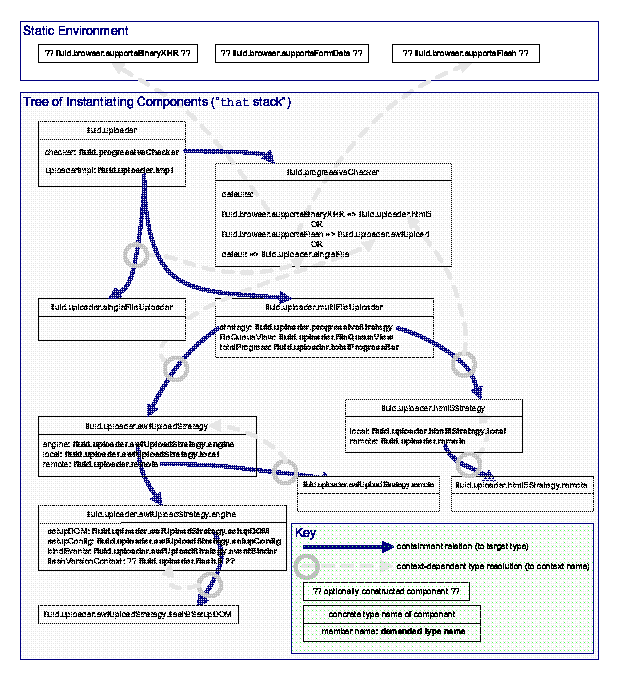
\includegraphics[width=6.185in]{uploader.eps}
\caption{Illustration of component tree instantiation for Uploader widget}
\label{fig:Uploader}
\end{figure*}
\subsubsection{Use of demands blocks in Uploader implementation}
Figure \ref{fig:Uploader} shows schematically the structure of some of the demands blocks implementing the Uploader widget. Each arrow linked with a circle along its length represents a {\it contextual resolution} --- a choice made by the instantiation system based on the context provided by constructions which have already concluded. At the top of the diagram are raw {\bf context tags} decoded by a direct inspection of the capabilities of the user agent --- {\tt fluid.browser.supportsBinaryXHR}, etc. Below this level in the tree is the point at which user configured material may be used to guide resolution, for a particular instantiation of the uploader, onto a particular strategy to be used. In the absence of this, the default demands structure will proceed by a default algorithm onto the uploader strategy tags, {\tt fluid.uploader.html5} etc. Below this level, the resolution continues to cascade onto particular elements of the uploader implementation, guided by the strategy tags. At each level of demands resolution, there is scope for further demands blocks contributed at the user's request, or an integrator or other party, to intercede, or in AOP terminology to ``advise'' the construction of subcomponents, by fetching data or implementation sourced from other parts of the uploader's tree --- or even, from other parts of a wider component tree. Whilst the uploader is packaged in such a way that it is usable by standard JavaScript citizens as a simple function call, the full power of the IoC system together with the uploader is only realised when the entire implementation of an application is delivered as a single, giant interconnected series of demands blocks --- with demands resolution given the power to roam freely and fetch contextualised data to be delivered anywhere within or among elements which would formerly have been seen to be opaque, monolithic ``components''.

Whilst Figure \ref{fig:Uploader} resembles a standard UML diagram in some respects, the meaning is somewhat different. This diagram shows a schematic for data structures which {\it might} exist in certain histories of the system, rather than those which will or do exist, statically. It is this contextual awareness at each point of the system that allows it to be easily extended for new cases, with instantiation guided along new paths, made visible by new demands blocks being brought into scope. 

\subsection{Wider case study - The CollectionSpace Collections Management System}

The CollectionSpace project\cite{collectionspace}, led by the Museum of the Moving Image in New York, is producing collections management software for the use of museum curators and other staff. The project is using the current version of the Infusion IoC system, as described here. This project is proving an excellent ground for exploring the benefits in adaptible and declarative software that the IoC approach can offer. The user interface for this application consists of few but very detailed pages, containing many hundreds of widgets, reflecting the level of detail of the specialised knowledge operated in the domain of exhibit curation. As suggested in the previous section, the entire UI for this application is implemented as a giant, single-rooted tree of components governed by the underlying graph of demands blocks. This tree comprises components such as the Uploader and numerous others, instantiated by IoC. One immediate benefit of this approach for users is the easy adaptibility of the interface in a schema-driven way. Rather than relying on development support to orchestrate changes required by local institutions which may have very widely differing requirements, these can instead be enacted by editing simply-structured JSON files or in many cases can be inferred automatically from a description of the application's schema.

Component markup, similar to component state, is not locked up in implementation files but ``out in the open'' in unpolluted and standard HTML files, reskinning of the application similarly can be performed without development support, using standard HTML editing tools. These kinds of reskinning comprise, but go beyond that possible through simple CSS effects. Directly editing HTML enables widespread reorganisation of the layout and content of the markup operated either by individual components or entire pages. This composition of markup is performed by the {\bf Fluid Renderer}, an engine described in more detail in the online references for the Fluid Framework.

\section{Status and Trajectory of the Implementation}

The Fluid group are currently working towards the 1.4 release of the Infusion system, which is targetted for the end of August 2011. This will be the first public release in which the described implementation of the IoC system (as well as the Uploader widget and other components not described here) will be available. This release is considered to be in a ``sneak peek'' mode where API and concepts are not fully stabilised. Although several of Fluid's production-ready components are implemented in terms of this system already, the IoC system and framework itself are not yet considered to have reached a production-worthy condition in terms of stable use by general users. Readers are invited to come along and inspect our progress, and even join in, at our github repository held at \url{https://github.com/fluid-project/infusion}\ . Overall documentation for the Infusion system, including the IoC implementation, is held at \url{http://wiki.fluidproject.org/display/fluid/Infusion+Documentation}\ . Future versions of Infusion are roadmapped at \url{http://wiki.fluidproject.org/display/fluid/Fluid+Community+Roadmaps} --- we will continue to stabilise and expand the capabilities of the IoC system as well as evolving previously implemented components to defer to it more for implementation. A crucially important, but still very early--stage work package involves our server-side implementation, Fluid {\bf Kettle}, an IoC-driven JavaScript implementation based on the rapidly developing {\tt Node.js} framework based on an asynchronous I/O model. A back-end based on Apache's CouchDB persistence technology using JavaScript as a query language will enable a homogeneous development model operating JavaScript at all tiers of the web application, which is hoped to bring developments of lowered barrier to entry by new developers as well as increased mobility of code and implementation algorithms between the layers. 

\subsection{Directions for the System}

We identify two important future directions and roles for the system, continuing from our discussion of Brooks\cite{brooks86}, which identifies a number of technical developments which might have the potential to increase the efficiency of development (see section \ref{sec:brooks}). 

\subsubsection{Graphical tools and environments}
The categories of {\it graphical programming} and {\it environments and tools} which Brooks identifies as crucial are ones which a constant motivation during the development of the system has been to facilitate. We expect work in them to be very fruitful. Brooks criticises the potential of graphical programming on two grounds which might remain relevant today --- firstly that ``flowcharts'' are a poor abstraction of software structure, and secondly that superimpositions of multiple views of a program's structure are unlikely to arrive at a properly synoptic view of its function, as one might expect from the correspondence between a VLSI chip's geometric structure and its function. 

We argue that the way software is designed must be modified, precisely to bring about such a correspondence between structure and function. Such structure must be built around the {\bf data} which is being manipulated on behalf of the user, as well as the direct {\bf interface} itself which is presented to manipulate this data. Rather than an abstract flowchart showing a sequence of operations expected to be performed by the machine, the user interface itself should be the focus of operations exposed to the user in expressing their intentions. Until the rules by which the user interface is constructed are specified in a declarative form open to interpretation by the system itself, rather than in opaque code only interpretable to a compiler, the {\it adaptible interface} required by Inclusive Design cannot be constructed (section \ref{sec:tower}). 

Similarly, organising parts of this adaptible interface directly around the sources, transformation steps, and sinks governing the user's data, brings this most vital part of the system close to its constituency of users, rather than deliberately setting out in the opposite direction as modern recommendations on {\it data hiding} propose. Structuring computation around data in publically named, structured units (section \ref{sec:state}) also promotes free restructuring of the actual algorithms which operate on it, making it easier to exploit variable availability of computing resources (for example, variable numbers of processors, or variable availability of computing power at different nodes of a client-server architecture). 

\subsubsection{``Automatic'' programming and expert systems}
\label{sec:parnas}

Brooks defines automatic programming as ``generation of a program for solving a problem from a statement of the problem specifications''. He cites Parnas \cite{parnas79} who reinterprets this goal as follows: {\it ``In short, automatic programming always has been a euphemism for programming with a higher-level language than was presently available to the programmer.''} Higher-level languages to date have been constructed in two directions. Firstly, ``bottom-up'', building on the base of lower-level languages in the directions developers consider desirable to increase their expressiveness - for example, the construction of languages such as C++ and Java from the base of C. Secondly, ``top-down'', deriving from an analysis of natural languages and vocabularies of users the kinds of computer languages their requirements might intelligibly expressed in --- this motivated the construction of the so-called ``fourth-generation languages'' (4GLs) such as MAPPER, Clipper, LiveCode, R and S. 

Bottom-up language developments often fail to successfully deliver more end user needs per quantum of developer effort, and are usually focussed towards needs in the developer's domain. Top-down language developments can be very successful within particular domains, but fail to build bridges {\it downwards} into the world of underlying developers, by creating an impenetrable {\bf abstraction boundary} at the level of the 4GL language syntax. Only by building a ``harmonious tower of abstractions'' as we allude to in section \ref{sec:tower} can we assist both kinds of community to cooperate harmoniously on the same design, and gain the scalability benefits needed to escape Brooks' curse. By building our system out of the JSON configuration naturally made available by builtin features of the JavaScript language, we avoid creating an impenetrable abstraction boundary of this kind, a boundary on either side of which the stakeholders speak mutually unintelligible languages.

We have described the similarities between the IoC resolution process and the ``goal-directed'' behaviour of inference engines such as those used in some expert systems (section \ref{sec:prolog}). We aim towards a system whereby the ``statement of problem specifications'' should simply be {\bf identified with} the ``program for solving a problem''.

\subsubsection{The Crucial Important of Homoiconicity}
\label{sec:tower}
Many of the benefits of Infusion IoC can be interpreted from the viewpoint of seeing its JSON dialect composed of defaults and demands blocks as a {\it Domain-Specific Language} (DSL) \cite{fowler2} enjoying a crucial property known as {\it homoiconicity}\cite{mcilroy}. Homoiconicity is a property of some programming languages, in which the primary representation of programs is also a conveniently expressed data structure of the language. This property makes it extremely easy to produce tools which {\bf transform} ``programs'' written in this language into other forms, as well as tools which enable graphical presentation and development of the program by developers and end users.

It is a crucial requirement of the goals of Inclusive Design that bridges can be built between the worlds of software professionals and users. Homoiconic characteristics of the base language are essential to allow a bidirectional transfer of artefacts between developers and end users who work with the finished product --- and allow these users to work from effects they see in the finished product back to their causes and thus conform them to their requirements. Without the transparency allowed by this bidirectional transfer, inclusive design becomes uneconomic, since each adaptation of the software must be pursued by {\it ad hoc} development.

In practice, the transfer from the world of software professionals to end users involves a tower of increasing levels of abstraction. In order for this transfer to be economical, the transfers should not be ``mutually blind'' but allow some form of harmonised understanding of the transferred abstraction --- that is, there should at no level in the system be an impenetrable abstraction boundary, through which the transfer of artefacts involves a complete loss of meaning. Homoiconicity of the base system is essential to such a ``harmonious tower of abstractions'', stretching from the low levels out into the world of users. Previous similar systems cast as DSLs, ``Fourth-generation languages'' (4GLs), or code generators (see section \ref{sec:parnas}) have failed to ensure this harmonious tower by introducing an impenetrable abstraction boundary represented by a language syntax.


\section{Conclusion}

We have made a case arguing that the longevity of application code, as well as the reach of its design space, is greatly increased by reducing as much of its volume as possible to a declarative form. A promising model for such a form are the JSON blocks we have described here, forming the demands and defaults blocks interpreted by the IoC-driven component system. We presented the feature of {\it homoiconicity} enjoyed by such code, expressed as natural data structures of the underling JavaScript language, as one of the crucial enablers of the application flexibility and scalable development required for Inclusive Design.

As platforms and technologies change, new demands blocks can weave together with the old to meet new needs, without fragility in existing implementations. Should \linebreak JavaScript and the web themselves cease to become current, this declarative form is easier to mechanically transform (following the mentality of LISP ``macros'') into forthcoming idioms, than implementations specified in imperative, sequential code. Such code that {\it is} written is packaged in global functions which are more or less ``free'', maximising the chance that it can be reused in fresh contexts without the worry of assumptions embodied in hazardous shared state such as that found in base classes or object instances. Finally, where expectations and contracts do change over time, old implementations may be adapted to new clients, and vice versa, by the interposition of suitable demands blocks, providing the appearance of new contracts for old.



% We recommend abbrvnat bibliography style.

\bibliographystyle{abbrvnat}

% The bibliography should be embedded for final submission.

\begin{thebibliography}{}
\softraggedright

\bibitem{lakos}
Lakos, J.:
Large-Scale C++ Software Design, 1996, Addison-Wesley Professional

\bibitem{mcilroy}
McIlroy, D.:
Macro Instruction Extensions of Compiler Languages, 1960, Communications of the ACM, Volume 3 Issue 4

\bibitem{inclusive-design}
Chapter 15: ``Everyday inclusive design'', N. Warburton, {\it in} Inclusive Design: Design for the whole population: Edited by Clarkson, J. et al, Springer (2003)

\bibitem{fowler}
Fowler, M.:
Inversion of Control Containers and the Dependency Injection pattern,
\url{http://martinfowler.com/articles/injection.html}

\bibitem{fowler2}
Fowler, M., Parsons, P:
Domain-Specific Languages, Addison-Wesley, 2010

\bibitem{crockford}
Douglas Crockford --- The JSON Saga: \url{http://developer.yahoo.com/yui/theater/video.php?v=crockford-json}

\bibitem{cop2005}
Pascal Costanza, Robert Hirschfeld, Language constructs for context-oriented programming: an overview of ContextL, in: DLS�05: Proceedings of the 2005 Symposium on Dynamic Languages, ACM, New York, NY, USA, 2005, pp. 1�10.

\bibitem{cop2009}
Malte Appeltauer, et al.: A Comparison of Context-oriented Programming Languages. In Proceedings of the Workshop on Context-oriented Programming (COP) 2009 Genoa, Italy, July 7, 2009

\bibitem{cop2010}
J. Lincke, et al. An open implementation for context-oriented layer composition in ContextJS, Science of Computer Programming (2010), doi:10.1016/j.scico.2010.11.013

\bibitem{functionpoints}
A. J. Albrecht: ``Measuring Application Development Productivity,'' Proceedings of the Joint SHARE, GUIDE, and IBM Application Development Symposium, Monterey, California, October 14�17, IBM Corporation (1979), pp. 83�92.

\bibitem{brooks86}
Brooks, Fred P.: ``No Silver Bullet � Essence and Accident in Software Engineering''. Proceedings of the IFIP Tenth World Computing Conference (1986): 1069�1076.

\bibitem{parnas79}
D.L. Parnas: ``Designing Software for Ease of Extension and Contraction,'' IEEE Transactions on Software Engineering, Vol. 5, No. 2, March 1979, pp. 128-38.

\bibitem{proxies}
ECMAScript 6 Proxy proposal:
\url{http://wiki.ecmascript.org/doku.php?id=harmony:proxies}

\bibitem{collectionspace}
The CollectionSpace Project: \url{http://www.collectionspace.org/}

\bibitem{gpii}
The Global Public Inclusive Infrastructure \url{http://www.gpii.org/}

\bibitem{rest}
Fielding, R.T.:
Architectural Styles and the Design of Network-based Software Architectures, Doctoral dissertation (2000), University of California, Irvine

\bibitem{martin}
Martin, J:
Managing the Data-base Environment, Prentice-Hall, 1983

\bibitem{pierce}
Pierce, B.C.:
Foundations for Bidirectional Programming, or: How To Build a Bidirectional Programming Language, June 2009. Keynote address at International Conference on Model Transformation (ICMT).

\bibitem{galois}
Kulkarni, M., Carribault, P., Pingali, K., Ramanarayanan, G., Walter, B., Bala, K., Chew, L.P.:
Scheduling strategies for optimistic parallel execution of irregular programs, SPAA '08 Proceedings of the {T}wentieth annual symposium on parallelism in algorithms and architectures

\bibitem{spring}
The Spring Framework, \url{http://www.springsource.org/about}

\bibitem{spring-security}
The Spring Security Framework, \url{http://static.springsource.org/spring-security/site/index.html}

\bibitem{jquery}
The jQuery Framework, \url{http://jquery.com}

\end{thebibliography}

\end{document}
